\begin{center}
\begin{tikzpicture}
    \node[anchor=south west,inner sep=0] (image)  at (0,0) {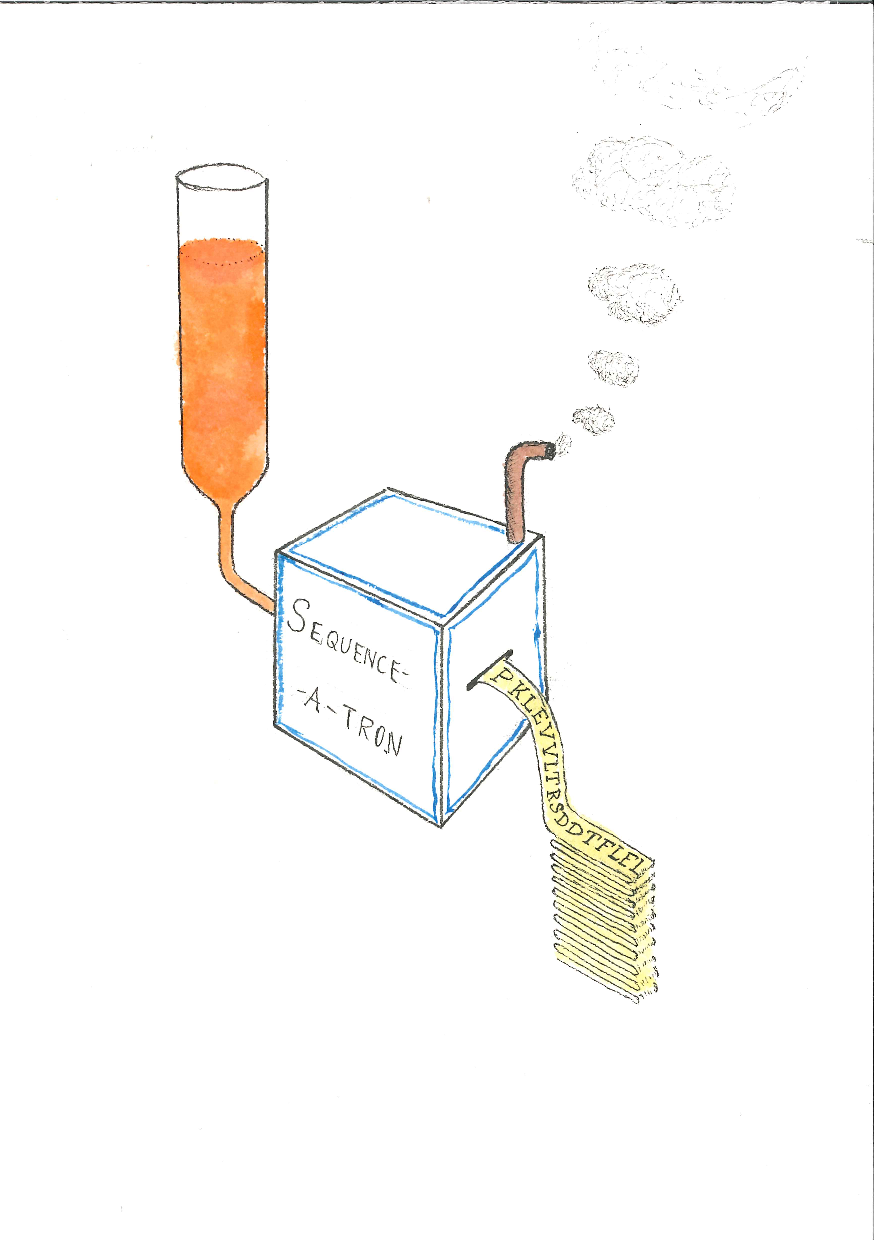
\includegraphics[trim={2mm, 2mm, 2mm, 2mm},width=0.995\pagewidth]{scans/pg_0001.pdf}};
    
    
    \begin{scope}[x={(image.south east)},y={(image.north west)}]
        \if\helplines1
        	\draw[help lines,xstep=.1,ystep=.1] (0,0) grid (1,1);
        \fi
        \node[align=justify, text width=0.4\pagewidth](en) at (0.7, 0.85) {\english{Performing an experiment to obtain the sequence of amino acids that form a protein is easy and straightforward.
        
        \doindent Nowadays, sequencing all the proteins of a human - a tad under hundred thousand - costs less than 1\,000 €.}};
        \node[align=justify, anchor=north west, text width=0.4\pagewidth](es) at (0.1, 0.3) {\spanish{Realizar el experimento para obtener la secuencia de aminoácidos que forman la proteína es fácil y sencillo.
        
        
        \doindent Hoy en día, secuenciar todas las proteínas de un humano - casi cien mil - cuesta menos de \oldstylenums{1\,000} €.}};
    \end{scope}
    
\end{tikzpicture}
\end{center}